\section{Polygonal Linkages}
A generalization of linkages is a polygonal linkage where edges of given lengths are replaced with rigid polygons.
Formally, a \textit{polygonal linkage} is an ordered pair $\left(\PP,\HH \right)$ where $\PP$ is a finite set of polygons and $\HH$ is a finite set of hinges; a \textit{hinge} $h\in \HH$ corresponds to two or more points on the boundary of distinct polygons in $\PP$.  
A \emph{realization of a polygonal linkage} is an interior-disjoint placement of congruent copies of the polygons in $\PP$ such that the copies of a hinge are mapped to the same point (e.g., Figure \ref{fig:linkage-1}).  
\begin{figure}[!htbp]
\begin{center}

\includegraphics[scale=1]{graphics/hingeOnThreeDistinctPolygons.pdf}
\end{center} 
\caption{(a) A polygonal linkage with a non-convex polygon and two hinge points corresponding to 
three polygons.  Note that hinge points correspond to two distinct polygons.(b) Illustrating that 
two hinge points can correspond to the same boundary point of a polygon.}
\label{fig:linkage-1}
\end{figure}
A \textit{realization of a polygonal linkage with fixed orientation} is a realization in which each polygon is translated and rotated copy of a polygon in $\PP$; at each hinge the incident polygons are in a given counter-clockwise order (refer to Figure \ref{fig:orderedLinkages}).
%the congruent copies of the polygons in $\PP$ is translated and rotated copy in $\PP$.
% each copy allows for any combination of translations and rotated copies of polygons in $\PP$ where every hinge has a counter-clockwise order of incident polygons.  
\begin{figure}[!htbp]\label{fig:orderedLinkages}
\begin{center}
\includegraphics[scale=1]{graphics/orderedLinkages.pdf}
\end{center} 
\caption{Two realizations of the same polygonal linkage with that differ in the counter-clockwise order of polygons around vertex $a$. }
\end{figure}
Note that oriented polygonal linkage realizations do not allow for reflection transformations of polygons in $\PP$.

These two realization types allow one to pose two different problems, the realizability problem for polygonal linkages and the realizability problem for polygonal linkages with fixed orientation:
\begin{prob}[Realizibility Problem for Polygonal Linkages]\label{problem:UnorderedPolygonal}
%The realizability problem for a polygonal linkage asks whether a given polygonal linkage has 
%a realization.
Given a polygonal linkage, does it have a realization?
\end{prob}
\begin{prob}[ Realizibility Problem for Polygonal Linkages with Fixed Orientation]\label{problem:OrderedPolygonal}
%The \emph{realizability} problem for a ordered polygonal linkage asks whether a given polygonal 
%linkage has a realization with respect to order.
Given a polygonal linkage with fixed orientation, does it have a realization?
\end{prob}
%Refer to Figure \ref{fig:orderedLinkages} to a polygonal link
Not every polygonal linkage has a realization.
\begin{figure}[!htbp]
\begin{center}
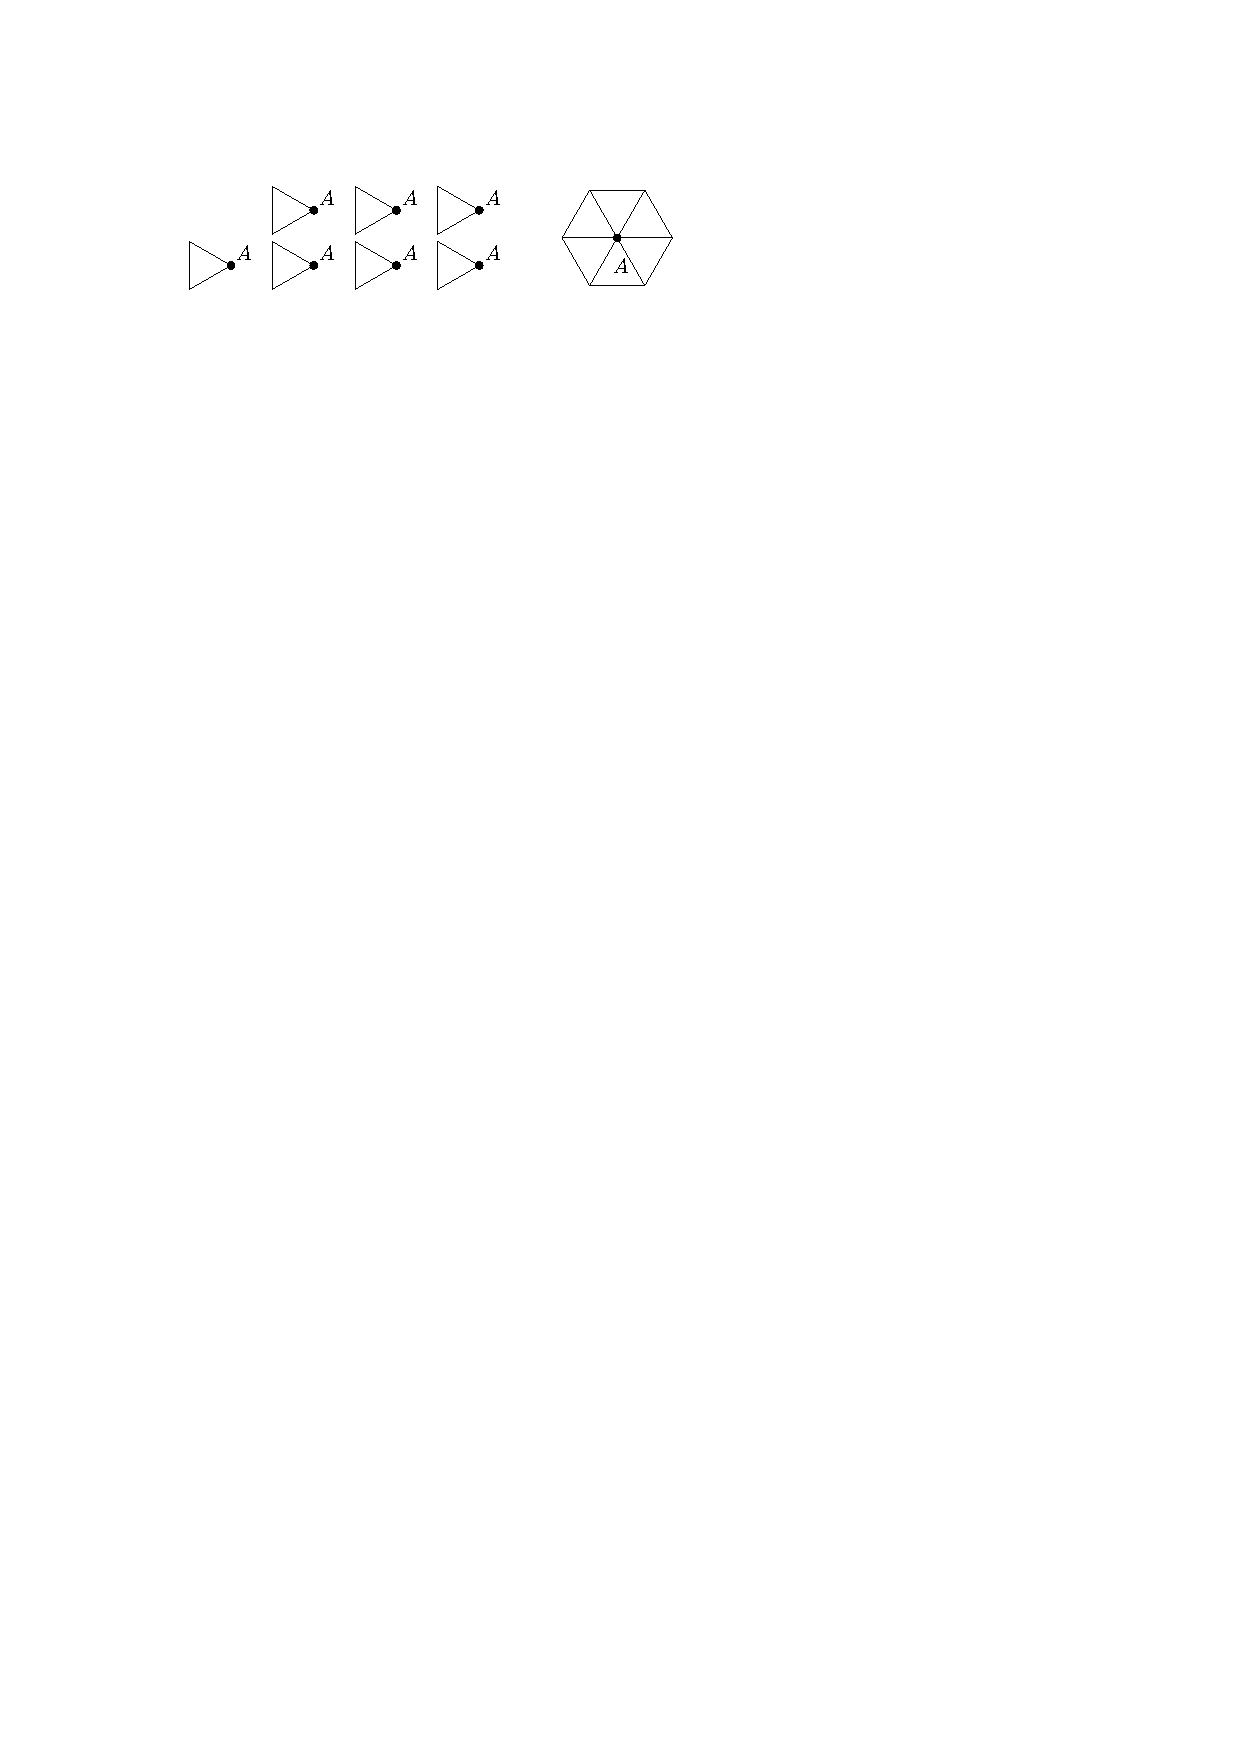
\includegraphics[scale=1]{graphics/Problem1.pdf}
\end{center} 
\caption{Here we have 7 congruent copies of an equilateral triangle with a hinge point of $A$.  The polygonal linkage is not realizable.  The best we can realize is at most 6 congruent copies of an equilateral triangle with the hinge point of $A$ in the plane.}
\label{fig:problem1}
\end{figure}
Consider the 7 congruent copies of an equilateral triange with a common hinge point in Figure \ref{fig:problem1}.
To show it does not have a realization, suppose it is realizable.  
Each angle of every triangle is $\frac{\pi}{3}$ radians.  
The sum of 7 angles formed by the triangles is $\frac{7\pi}{3}>2\pi$.  
The total radian measure around $A$ is $2 \pi$.
%In an interior disjoint placement of the triangles, the sum of angles incident at any point is at most $2\pi$.
The contradiction is that the sum of 7 angles formed by the triangles in an interior disjoint placement is $\frac{7\pi}{3}$.
%This exceeds the total radian measure around $A$ and so we cannot have a realization.
The polygonal linkage of Figure \ref{fig:problem1} would overlap itself and does not have a realization.

There are polygonal linkages that admit realizations but every realization requires rotation.
Figure \ref{fig:collidingHingedPolygons} show the congruent copies of the polygons $A$, $B$, $C$, and $D$ in two different configurations, the far right is a realization, the middle fails to be a realization because of the interiors of $B$ and $D$ intersecting and the left showing the polygons in $\PP$.  
In fact, this polygonal linkage cannot admit a realization with fixed orientation.
Indeed this polygonal linkage cannot satisfy Problem \ref{problem:OrderedPolygonal}, suppose there is a realization with fixed orientation.  
Without loss of generality, fix the placement of $C$.
$A$, $B$, and $D$ have unique placement around triangle $C$.  
In this placement $C$ and $D$ overlap.%have common intersecting interiors and thus a contradiction of the existence of a realization.  
\begin{figure}[!htbp]\label{fig:collidingHingedPolygons}
\begin{center}
\includegraphics[scale=1]{graphics/collidingHingedPolygons.pdf}
\end{center} 
\caption{This example shows yet another example where two realizations of the same polygonal linkage. 
 One realization where there is an intersection and another where there isn't an intersection.}
\end{figure}
Figure \ref{fig:collidingHingedPolygons}, satisfies Problem \ref{problem:UnorderedPolygonal} but not Problem \ref{problem:OrderedPolygonal}.
 The far right is a realization but with polygon $B$ reflected.
  %If $B$ were not reflected we see that the only way to attach the polygons by their hinges together is if $B$ and $D$ intersect in their interiors.  

Figure \ref{fig:collidingHingedPolygons} does not quite get at the heart of the challenge with Problem \ref{problem:UnorderedPolygonal} because the counter-clockwise order of the polygons around hinges is not considered.
\begin{figure}[!htbp]\label{fig:orderedFaces.pdf}
\begin{center}
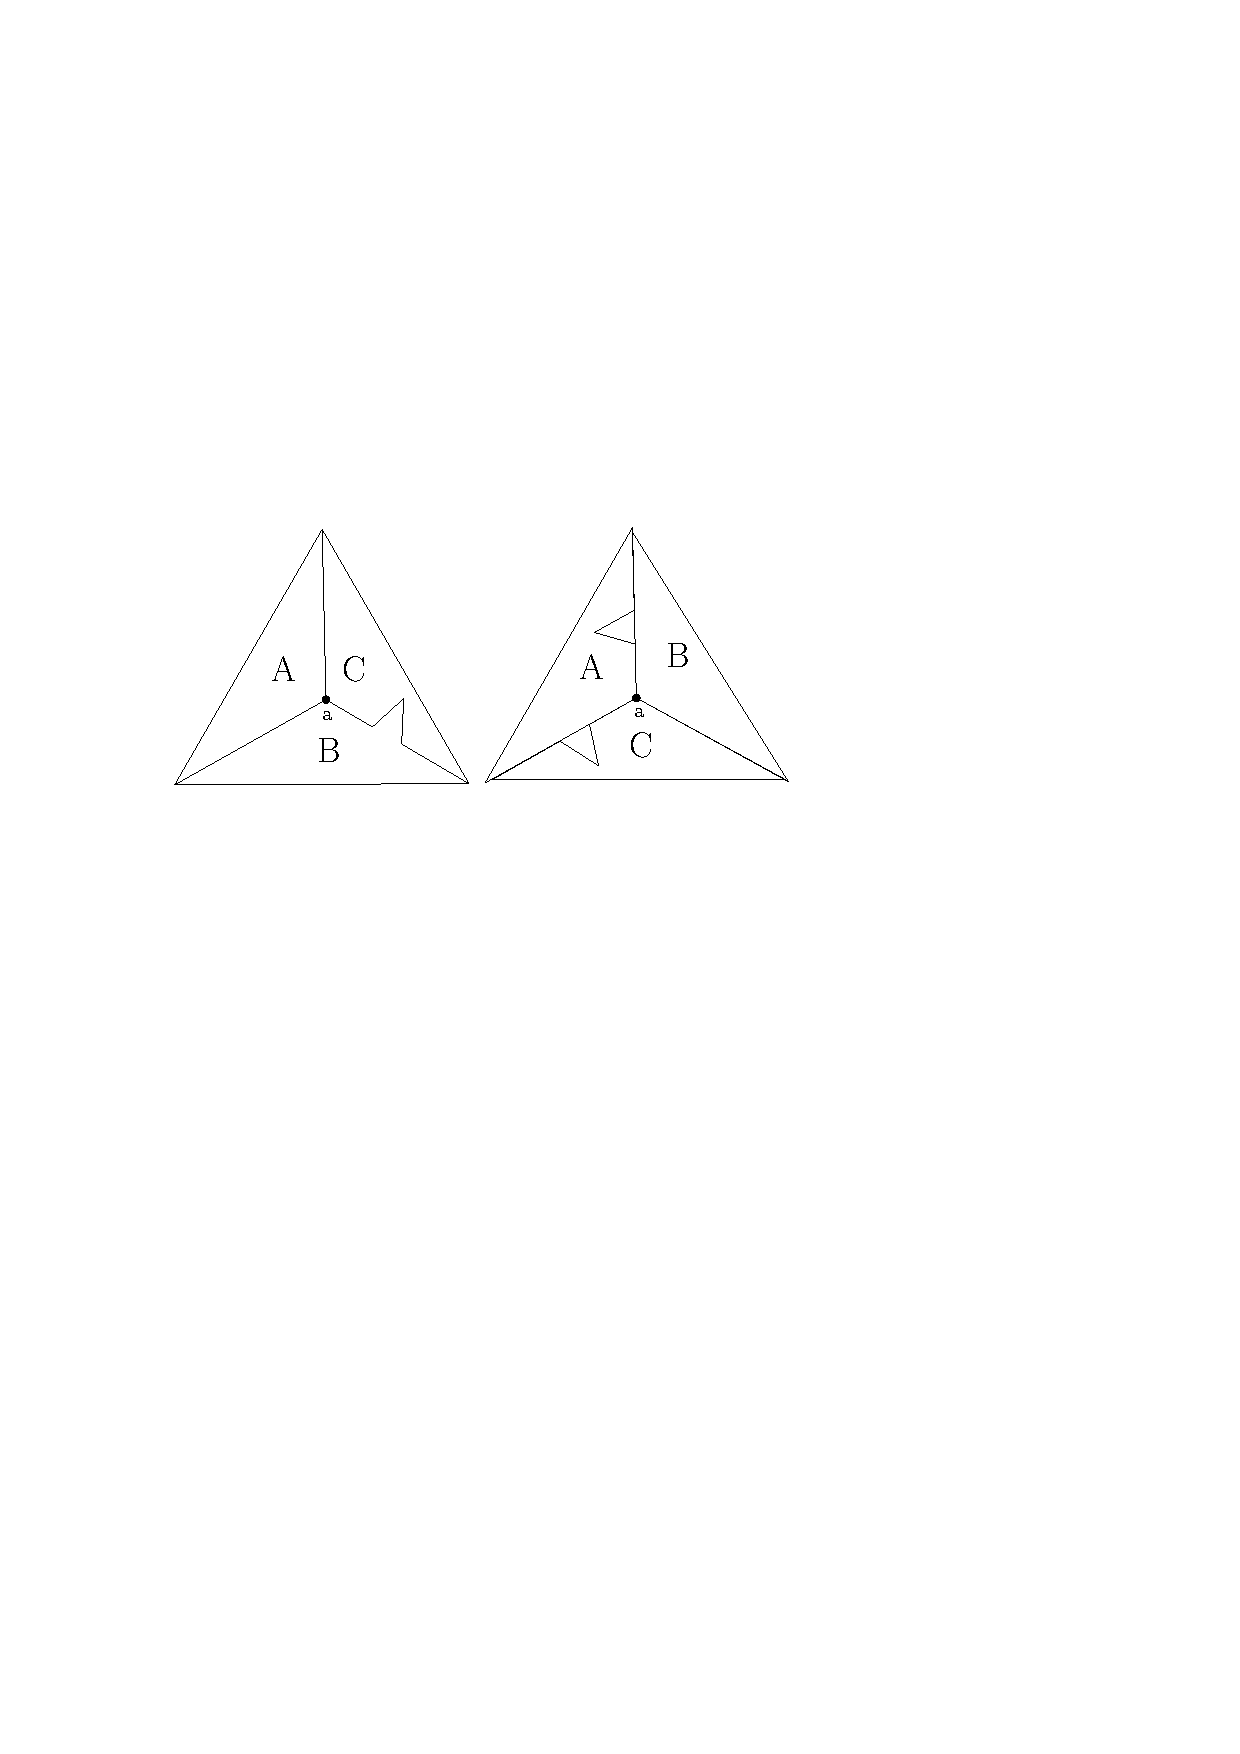
\includegraphics[scale=1]{graphics/orderedFaces.pdf}
\caption{Here we have two realizations of a polygonal linkage with two different counter-clockwise order (C,B,A) and (B,C,A) respectively.  
Note that the placement with ordering (B,C,A) has an overlap.}
\end{center} 
\end{figure}

Figure \ref{fig:orderedFaces.pdf} shows three polygons with a common hinge.
In the counter-clockwise order $(A,B,C)$, the polygonal linkage admits a realization whereas in the counter-clockwise order $(A,C,B)$, it does not admit a realization.
The examples above show that answers to Problem \ref{problem:UnorderedPolygonal} and \ref{problem:OrderedPolygonal} could be yes or no; the answer could be negative for various reasons.
Sections 2 and 3 of this thesis address the computational complexity of solving Problems \ref{problem:UnorderedPolygonal} and \ref{problem:OrderedPolygonal}.
We show that both problems are intractable.




\subsection{Geometric Dissections}
Hilbert's third problem asks: given any two polyhedra of equal volume, is it always possible to cut the first into finitely many polyhedral pieces which can be reassembled to yield the second \cite{aigner2010hilbert}?  
In three dimensions the answer is no however for two dimensions it is true \cite{10.23073621846}.

The Wallace-Bolyai-Gerwien Theorem simply states that two polygons are congruent by dissection iff they have the same area.  
A \textit{dissection} being a collection of smaller polygons whose interior disjoint union forms a polygon.
Hinged dissections of a polygon $P$ is a polygonal linkage that admits a realization that forms $P$.  
%The question of given two polygons of equal area, does there exist a hinged dissection whose two possible realizations are the polygons?
Demaine et. al. \cite{abbott2012hinged} showed that any two polygons of the same area have a common hinged dissection where polygonal pieces must hinge together at vertices to form a connected realization and that there exists a continuous motion between the two realizations (refer to section 1.5.3).
The was an outstanding problem for many years until 2007.

The Haberdasher Puzzle was proposed in 1902 by Henry Dudeney: can a square and an equilateral triangle of the same area have a common dissection into four pieces? 
%%%add story about the puzzle%%%%

\begin{minipage}
\begin{center}
\includegraphics{graphics/HaberdasherProblem.pdf}
\end{center}
\caption{figure}{The Haberdasher Puzzle was proposed in 1902 and solved in 1903 by Henry Dudeny.  The dissection is for polygons that forms a square and equilateral traingle
 }
\label{fig:polygonallinkage-5}
\end{minipage}

Geometric dissections are closely related to polygonal linkages.  
Figure \ref{fig:polygonallinkage-4} shows two arrangements of the same polygons to form a hexagon and a square. 
The polygons are not hinged and are arranged in differing order.
The polygons are merely tiled together to form the hexagon and square. 

\begin{minipage}
\begin{center}
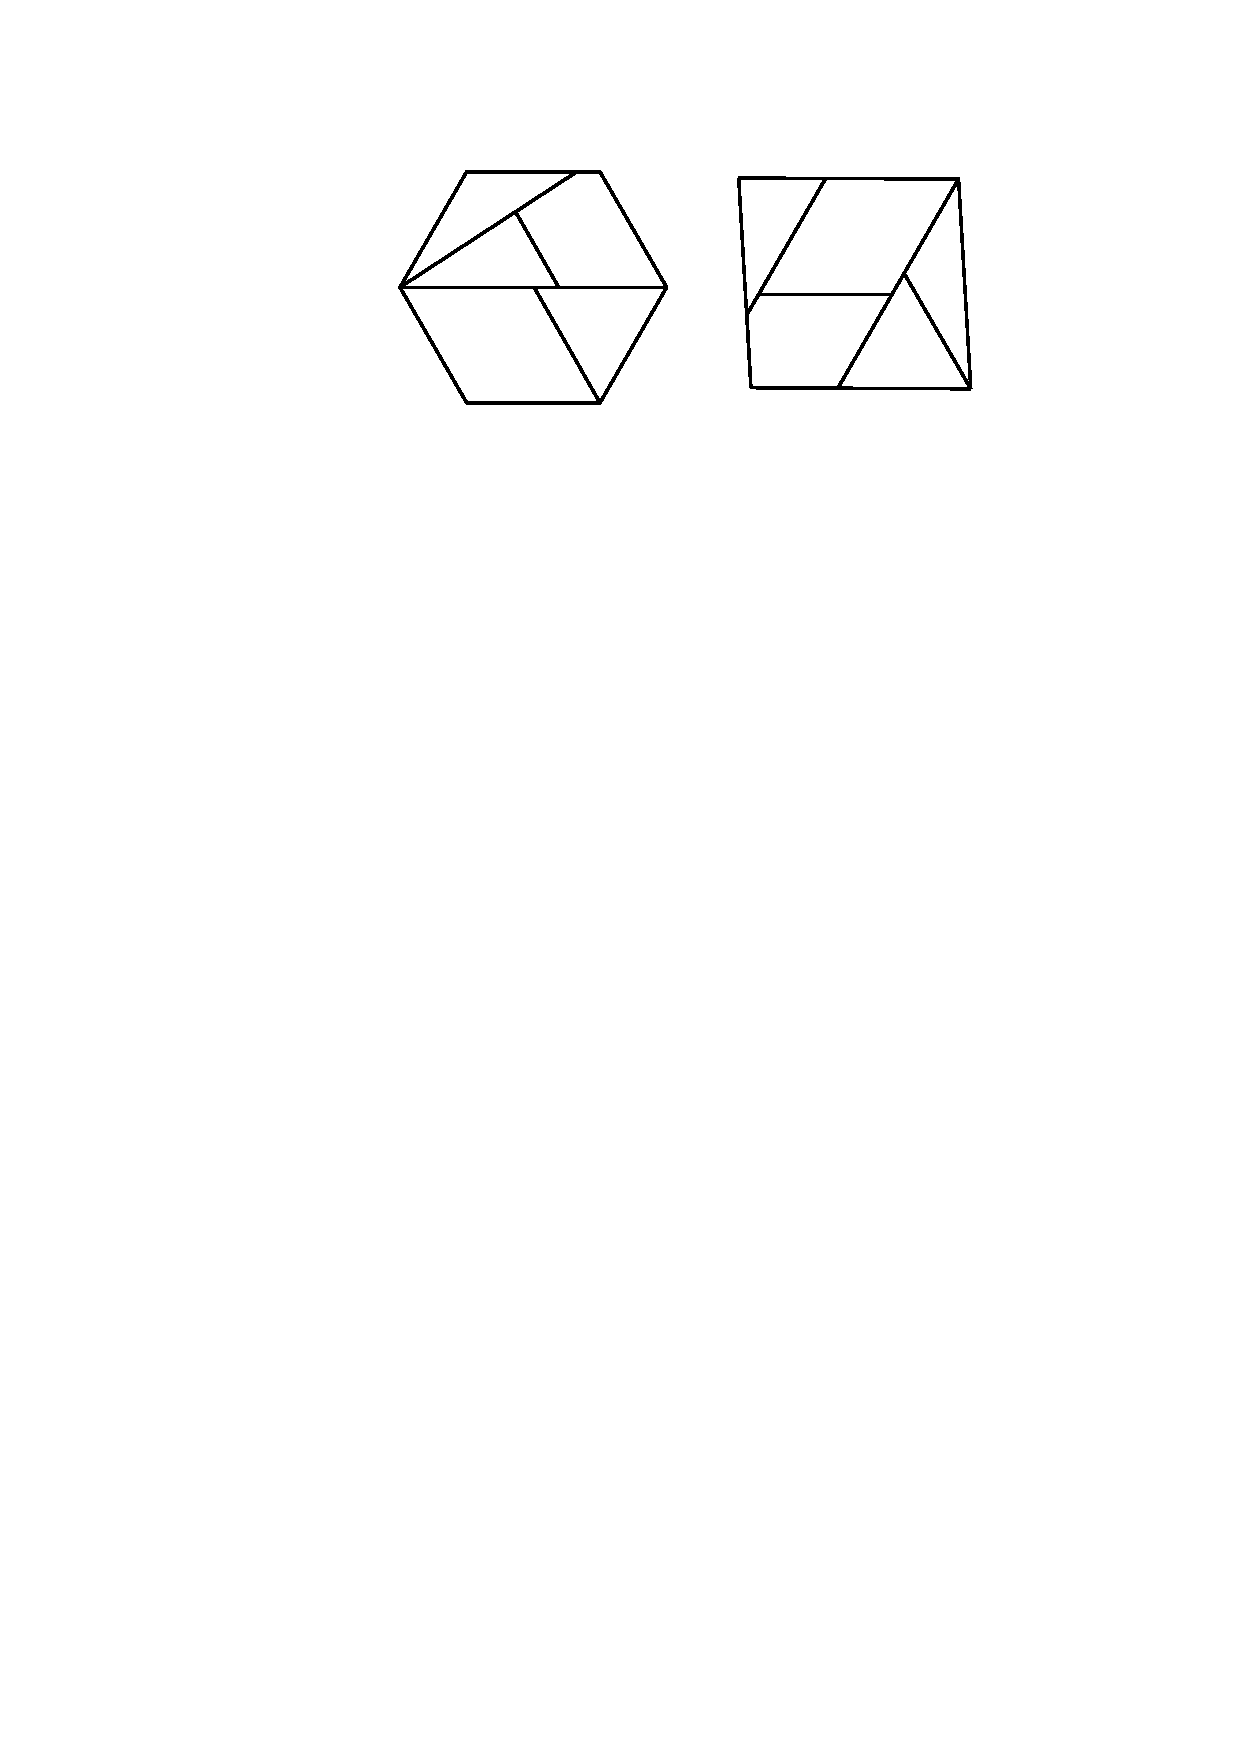
\includegraphics{graphics/GeometricDissectionBusschop.pdf}
\end{center}
\caption{figure}{Two configurations of polygonal linkage where the polygons touch on boundary segments 
instead of hinges.  These two realizations of the polygonal linkage are invalid to our definitions. 
 }
\label{fig:polygonallinkage-4}
\end{minipage}

Figure \ref{fig:HingedHaberdasher}, shows the Haberdasher problem with hinges.  
This makes the Haberdasher problem as a type of polygonal linkage where the polygons are free to move about their hinge points and take the form of a triangle or square.  

\begin{minipage}[!htbp]
\begin{center}
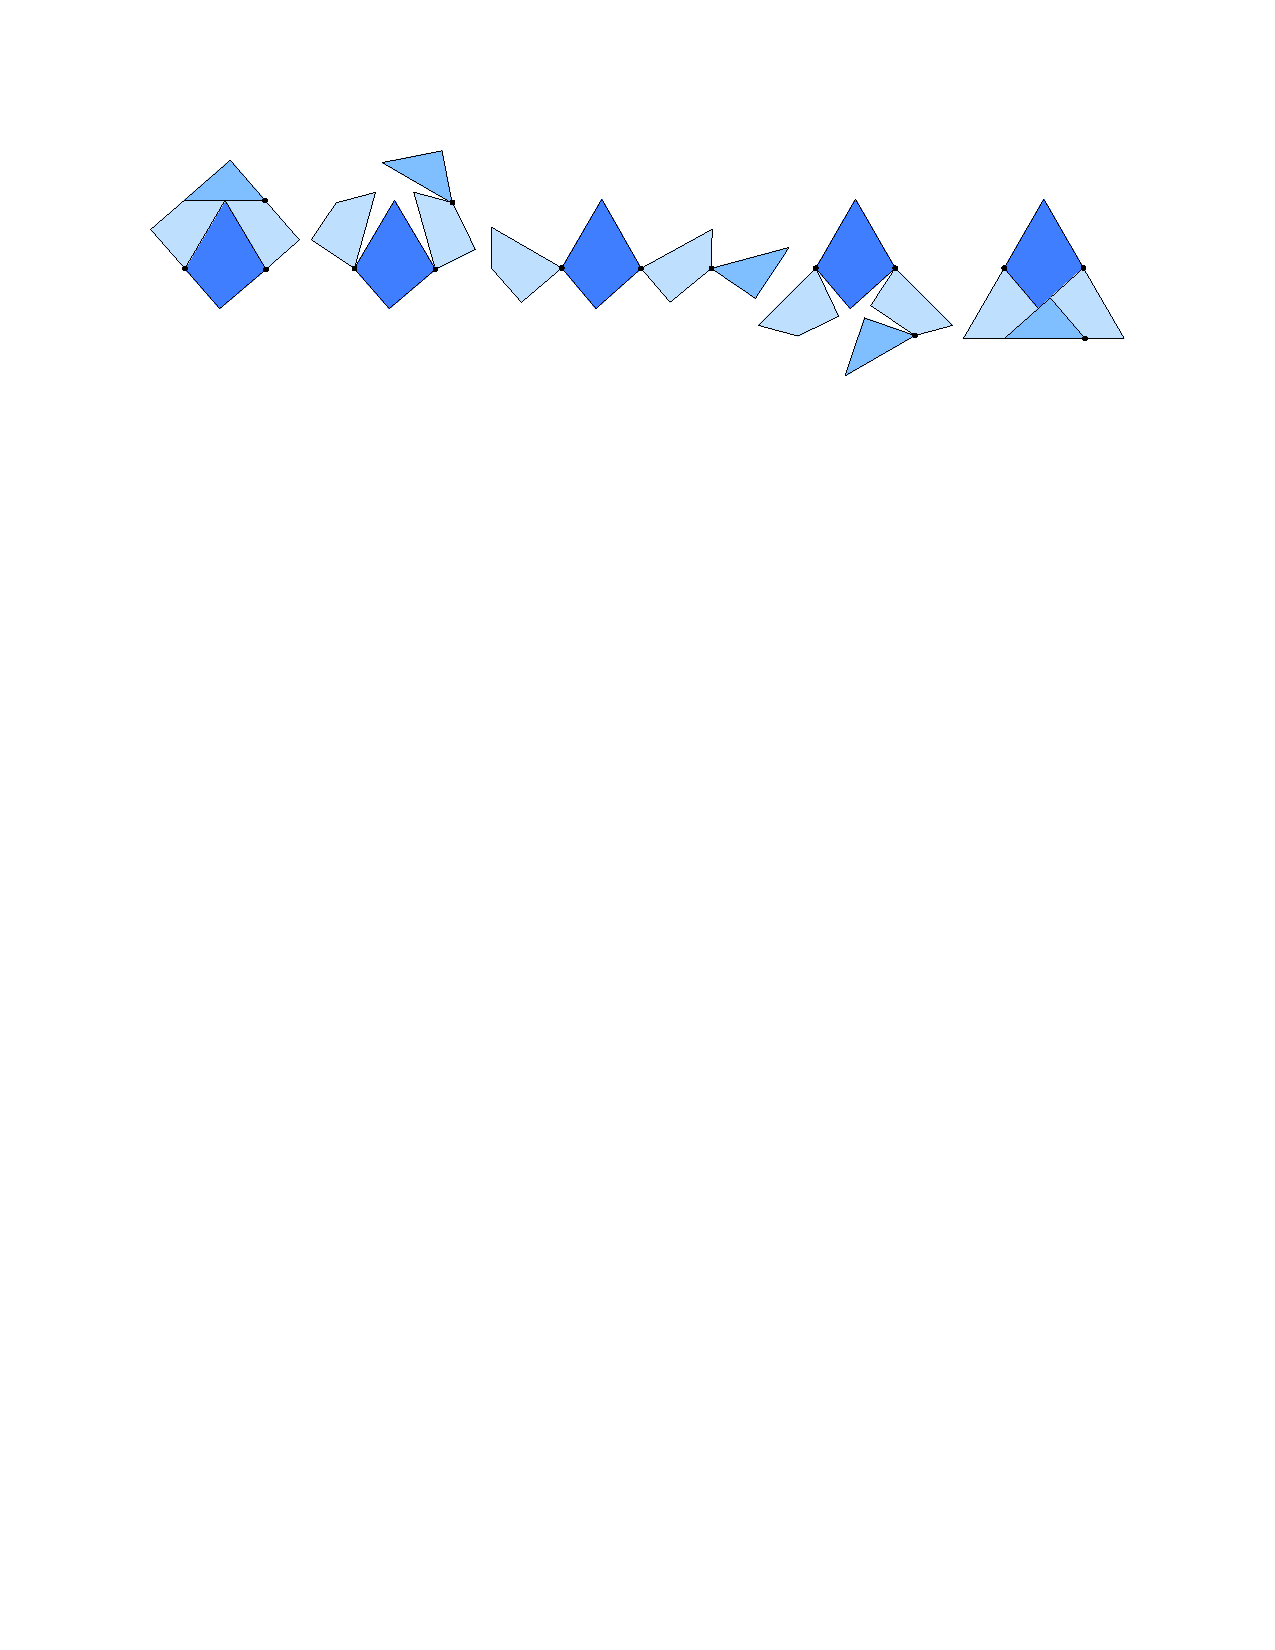
\includegraphics[width=\textwidth]{graphics/HingedHaberdasher.pdf}
\end{center}
\caption{figure}{This shows the Haberdasher problem in the form of polygonal linkage \cite{abbott2012hinged}.  This is a classic example of two polygons of equal area that have a common hinged dissection.}
\label{fig:HingedHaberdasher}
\end{minipage}




% With three cuts, dissect an equilateral triangle into a square. The problem was first proposed by Dudeney in 1902, and subsequently discussed in Dudeney (1958), and Gardner (1961, p. 34), Stewart (1987, p. 169), and Wells (1991, pp. 61-62). The solution can be hinged so that the four pieces collapse into either the triangle or the square. Two of the hinges bisect sides of the triangle, while the third hinge and the corner of the large piece on the base cut the base in the approximate ratio 0.982:2:1.018.



% %%%%%%%%%%%%%%%%%%%%%%%%%%%%%%%%%%%%%%%%%%%%%%%%%%%%%%%%%%%%%%%%%%%%
% %%%%%%%%%%%%%%%%%%%%%%%%%%%%%%%%%%%%%%%%%%%%%%%%%%%%%%%%%%%%%%%%%%%%
% %%%%%%%%%%%%%%%%%%%%%%%%%%%%%%%%%%%%%%%%%%%%%%%%%%%%%%%%%%%%%%%%%%%%
% %%%%%%%%%%%%%%%%%%%%%%%%%%%%%%%%%%%%%%%%%%%%%%%%%%%%%%%%%%%%%%%%%%%%
% %%%%%%%%%%%%%%%%%%%%%%%%%%%%%%%%%%%%%%%%%%%%%%%%%%%%%%%%%%%%%%%%%%%%
% %%%%%%%%%%%%%%%%%%%%%%%%%%%%%%%%%%%%%%%%%%%%%%%%%%%%%%%%%%%%%%%%%%%%
% %%%%%%%%%%%%%%%%%%%%%%%%%%%%%%%%%%%%%%%%%%%%%%%%%%%%%%%%%%%%%%%%%%%%
% \begin{figure}[h]
% \begin{center}
% 
\includegraphics[scale=1]{graphics/hingeOnThreeDistinctPolygons.pdf}
% \end{center} 
% \caption{(a) A polygonal linkage with a non-convex polygon and two hinge points corresponding to 
% three polygons.  Note that hinge points correspond to two distinct polygons.(b) Illustrating that 
% two hinge points can correspond to the same boundary point of a polygon.}
% \label{fig:linkage-1}
% \end{figure}
% %describe how it is a generalization of Linkages.
% A generalization of linkages are polygonal linkages where the edges of given lengths are replaced 
% by rigid polygons.  Formally, a \textit{polygonal linkage} is an ordered pair $\left(\PP,\HH 
% \right)$ where $\PP$ is a finite set of polygons and $\HH$ is a finite set of hinges; a 
% \textit{hinge} $h\in \HH$ 
% corresponds to two points on the boundary of two distinct polygons in $\PP$.  A \emph{realization} 
% of a polygonal linkage is an interior-disjoint placement of 
% congruent copies of the polygons in $\PP$ such that the points corresponding to each hinge are 
% identified (Fig. \ref{fig:1}). 
% A \textbf{realization with orientation} uses only translated or rotated copies of the polygons in $\PP$ (no reflections) and for each hinge, the cyclic order of incident polygons is given. 
% The topology of a polygonal linkage can be represented by the \textbf{hinge graph}, a bipartite graph where the vertices correspond to polygons in $\PP$ and the hinges in $H$, and edges represent the polygon-hinge incidences.
% This definition of realization rules well known geometric 
% dissections (e.g. Fig. \ref{fig:polygonallinkage-4}).
% %this is where the geometric dissection figure belongs
% \begin{figure}[h]
% \begin{center}
% 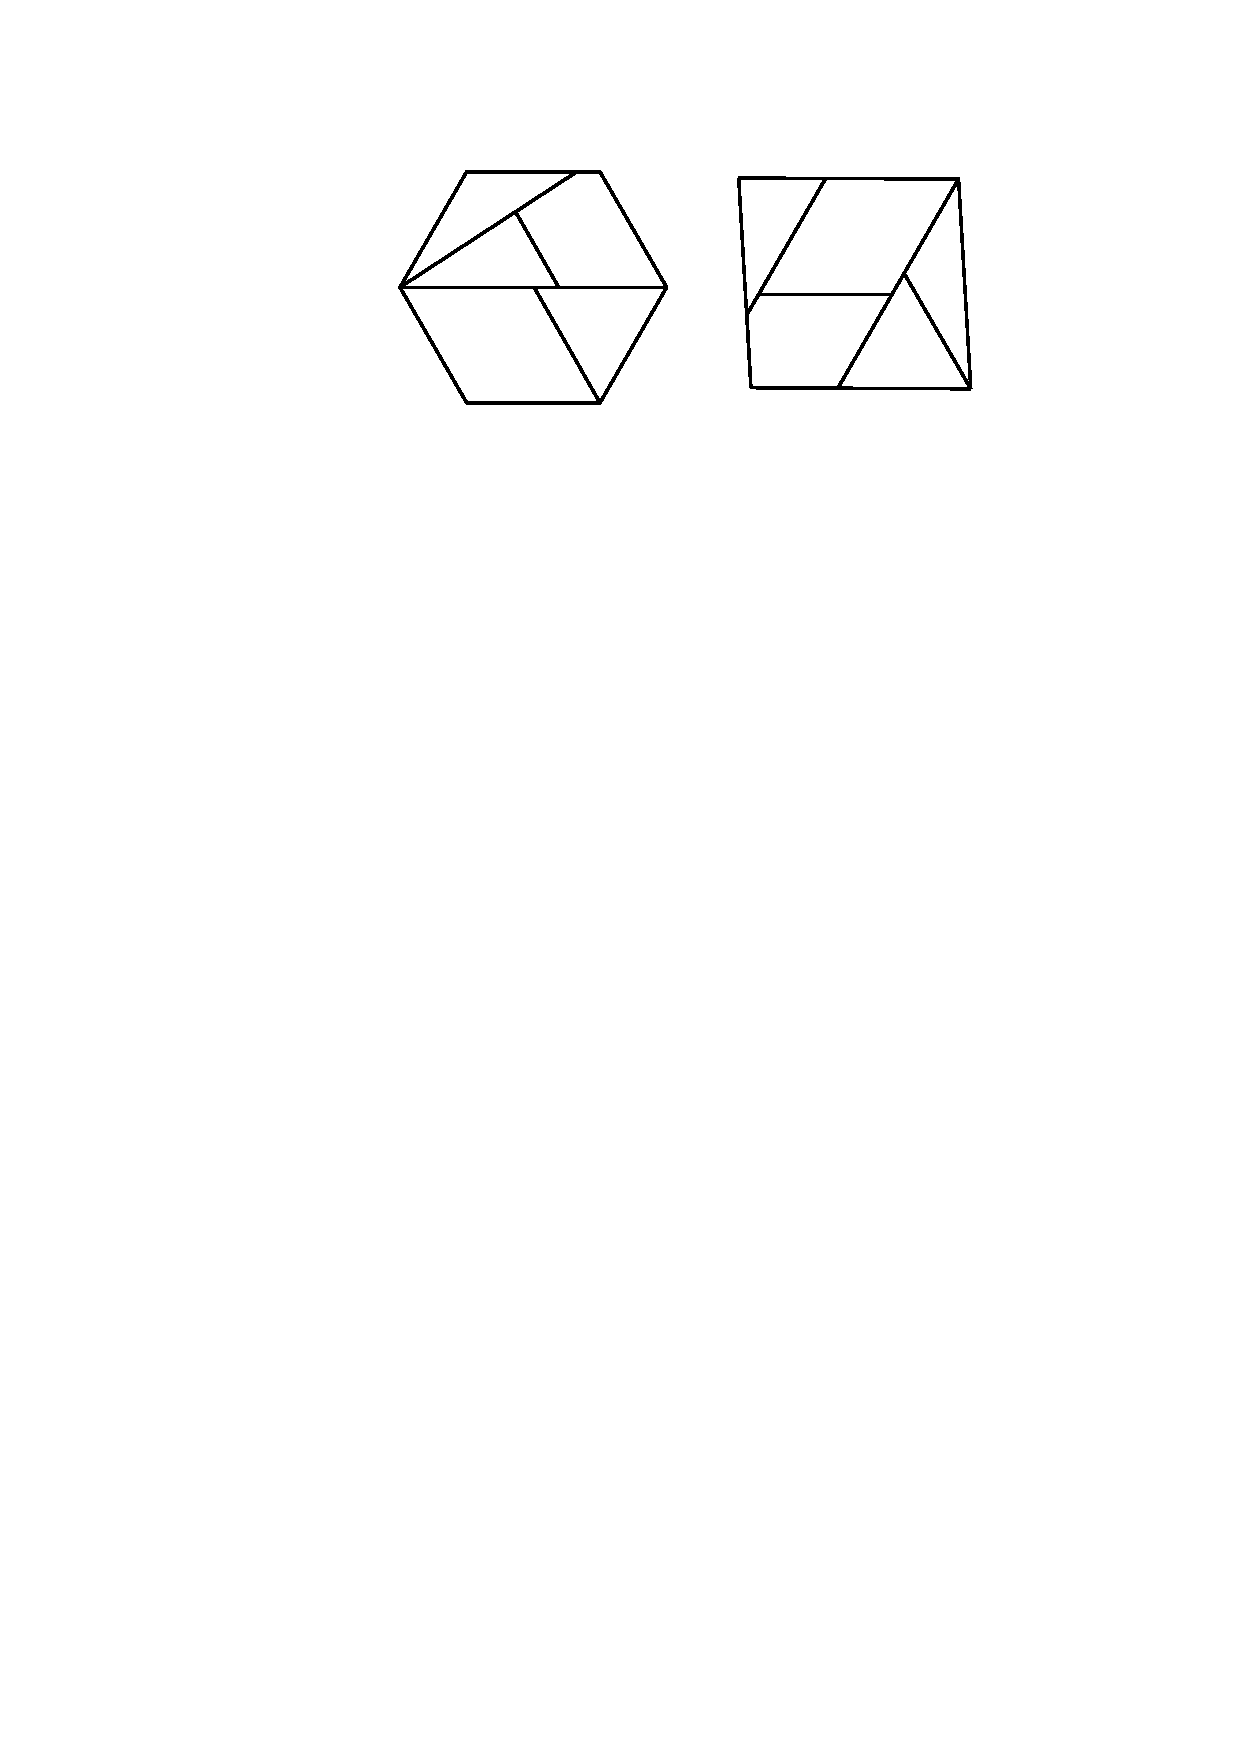
\includegraphics{graphics/GeometricDissectionBusschop.pdf}
% \end{center}
% \caption{Two configurations of polygonal linkage where the polygons touch on boundary segments 
% instead of hinges.  These two realizations of the polygonal linkage are invalid to our definitions. 
%  }
% \label{fig:polygonallinkage-4}
% \end{figure}

% \begin{figure}[h]
% \begin{center}
% 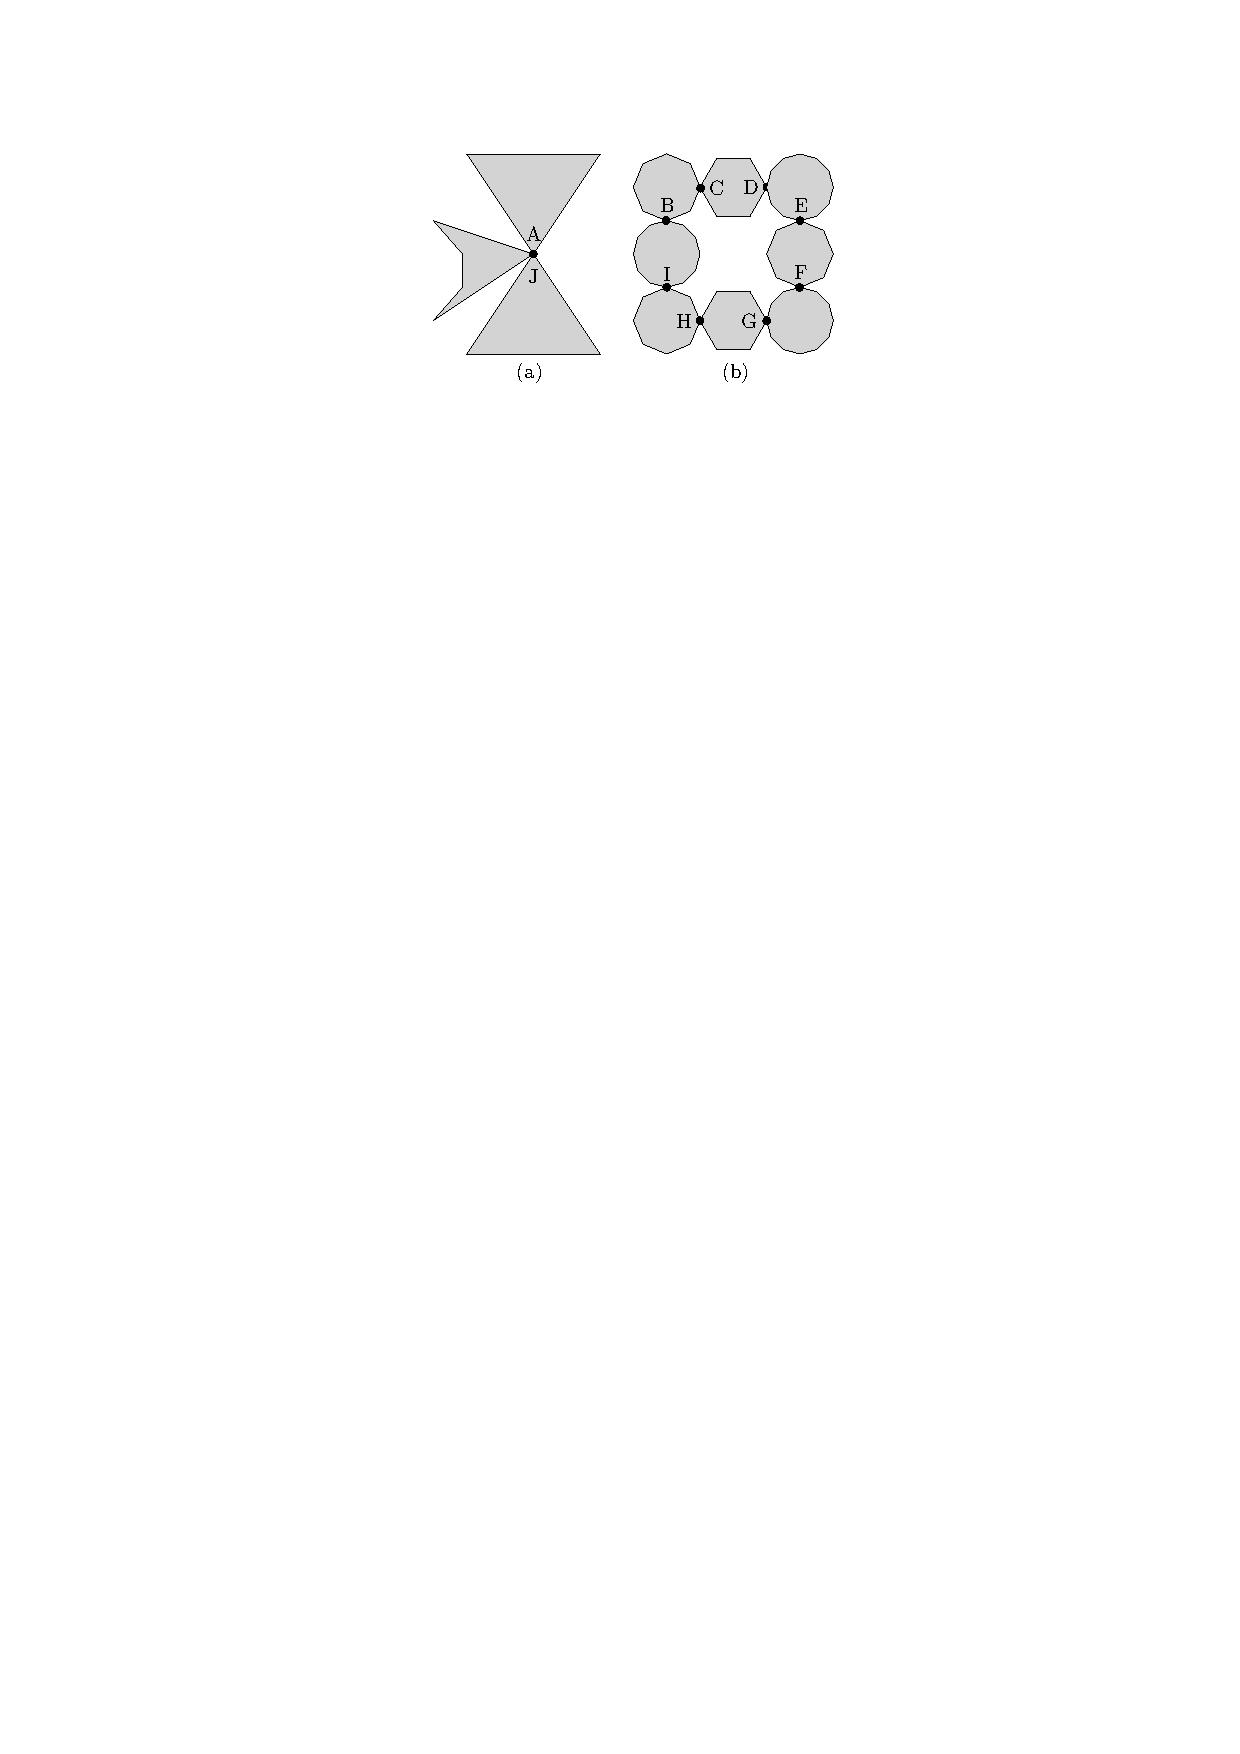
\includegraphics[scale=1]{graphics/linkageillustration.pdf}
% \end{center} 
% \caption{(a) A polygonal linkage with a non-convex polygon and a hinge point corresponding to three 
% polygons.  (b) A polygonal linkage with 8 regular polygons.}
% \label{fig:linkage-2}
% \end{figure}
% %%%%%%%%%%%%%%%%%%%%%%%%%%%%%%%%%%%%%%%%%%%%%%%%%%%%%%%%%%%%%%%%%%%%
% %%%%%%%%%%%%%%%%%%%%%%%%%%%%%%%%%%%%%%%%%%%%%%%%%%%%%%%%%%%%%%%%%%%%
% %%%%%%%%%%%%%%%%%%%%%%%%%%%%%%%%%%%%%%%%%%%%%%%%%%%%%%%%%%%%%%%%%%%%
% %%%%%%%%%%%%%%%%%%%%%%%%%%%%%%%%%%%%%%%%%%%%%%%%%%%%%%%%%%%%%%%%%%%%
% %%%%%%%%%%%%%%%%%%%%%%%%%%%%%%%%%%%%%%%%%%%%%%%%%%%%%%%%%%%%%%%%%%%%
% %%%%%%%%%%%%%%%%%%%%%%%%%%%%%%%%%%%%%%%%%%%%%%%%%%%%%%%%%%%%%%%%%%%%
% %%%%%%%%%%%%%%%%%%%%%%%%%%%%%%%%%%%%%%%%%%%%%%%%%%%%%%%%%%%%%%%%%%%%

% For the remainder of this thesis, we'll focus on the polygonal linkages with the following 
% restrictions:
% \begin{enumerate}
% \item Embedded polygons must be convex, i.e. for any two embedded points $u,v \in P'$, the set:
% $$\left\lbrace u  \cdot t + (1-t) \cdot v : t \in [0,1] \right\rbrace \in P'$$
%  \item  Polygons can only intersect at hinge points.  No two polygons can intersect at 
% their boundary or interior with the exception of possible a hinge point.  
% \end{enumerate}